\section{Architettura Transformer}

\begin{figure}[H]
    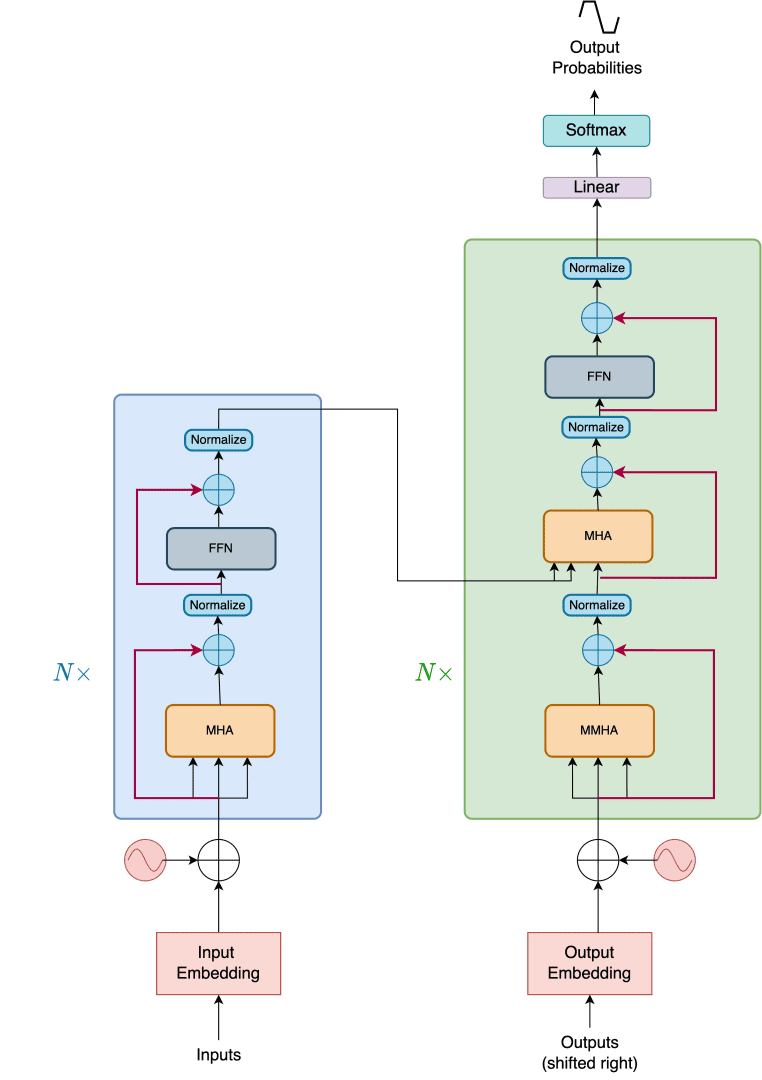
\includegraphics[width=\textwidth]{images/entire-architecture.png}
    \caption{Architettura Transformer}
\end{figure}

\begin{definition}(Attention)
    L'Attention è un meccanismo che assegna un peso a
    ogni parte dell'input durante il processo di elaborazione
    di un modello Transformer. Questi pesi determinano quanto ogni
    parte dell'input contribuisce all'output. Matematicamente,
    l'Attention può essere definita come una funzione $f$ che
    prende in input una query $q$, un insieme di coppie chiave-valore
    $(k, v)$, e restituisce un output $o$ calcolato come una somma pesata dei valori
    $v$, dove i pesi sono determinati dalla compatibilità tra la query $q$ e
    le chiavi $k$.
\end{definition}

\subsection{Multihead Attention}

\begin{figure}[H]
    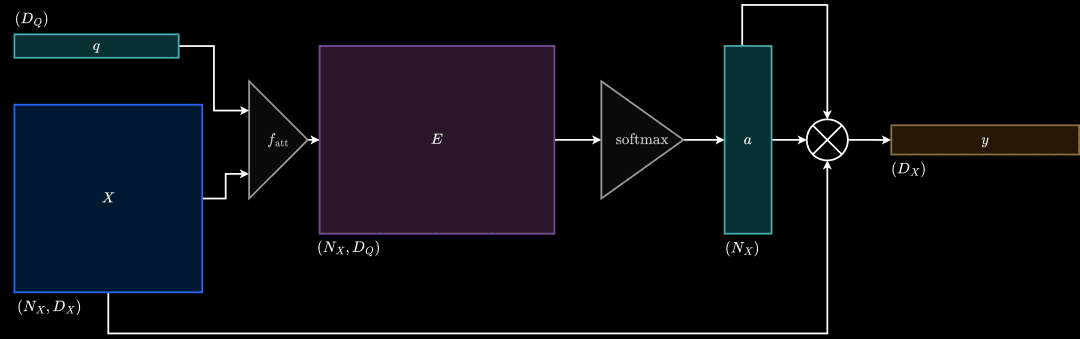
\includegraphics[width=\textwidth]{images/evolution-Version-0.png}
    \caption{Multihead Attention Versione 0}
\end{figure}

\textbf{fatt}: F-attention è la rete dove ci sono i parametri che vanno allenati per questa architettura. Tutto quanto
risiede in questo punto.

Ma ci sono state altre versioni per questa architettura. La versione 0 è quella
che abbiamo visto prima. La versione 1 è praticamente una versione che ha $D_Q$
fissato. Sparisce la \textbf{fatt} e quindi sparisce la rete neurale in questa
architettura.

\begin{figure}[H]
    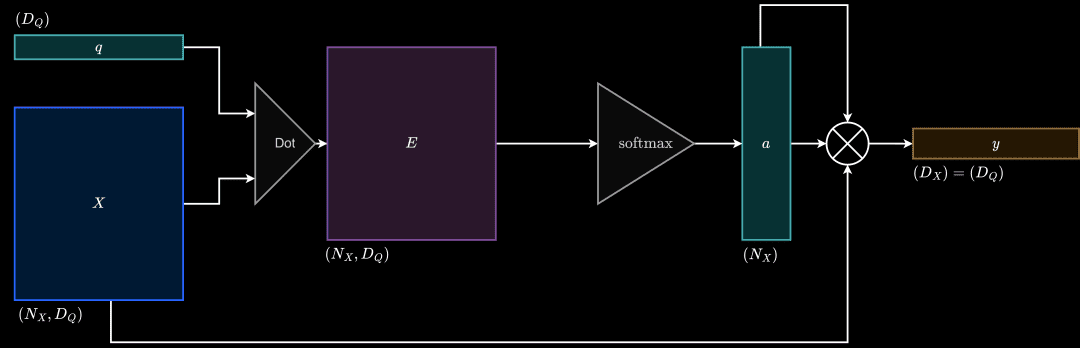
\includegraphics[width=\textwidth]{images/evolution-Version-1.png}
    \caption{Multihead Attention Versione 1}
\end{figure}

Anche questa soluzione, però, non funziona nel mondo reale. Serve fare qualche
altro cambiamento.

\begin{figure}[H]
    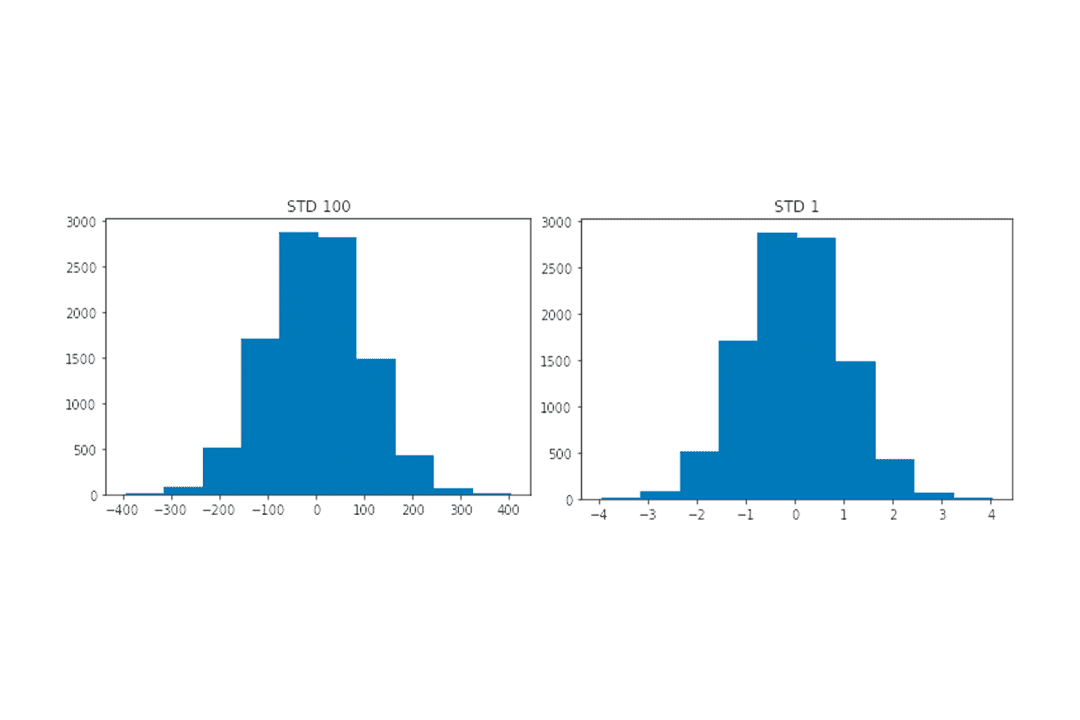
\includegraphics[width=\textwidth]{images/un-softmax-sol-diagram.png}
    \caption{STD Difference}
\end{figure}

In questo grafico si vedono 2 distribuzioni simili, ma che hanno una campana
una più piccola e una più larga. Questo dipenede dalla \textbf{Deviazione
    Standard}. Cosa entra in gioco in questo caso? $Softmax$. Se si fa il plot
della softmax, si vede che normalizzare permette di avere una scala.

\begin{figure}[H]
    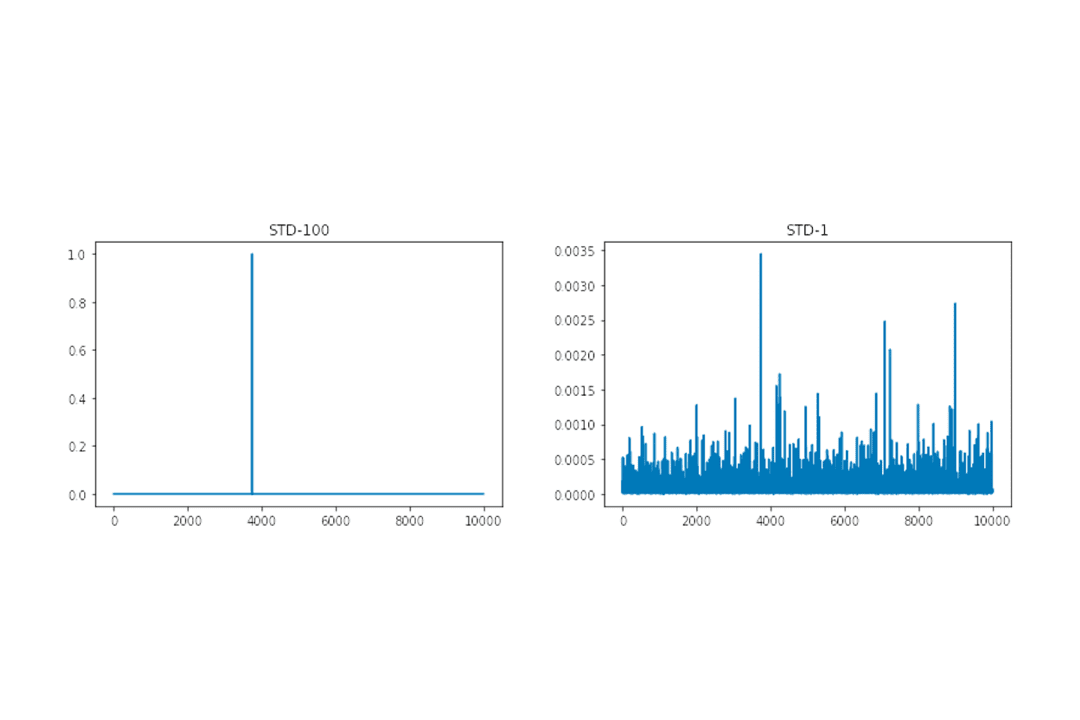
\includegraphics[width=\textwidth]{images/softmax-std-diagram.png}
    \caption{Softmax Plot}
\end{figure}

Come vediamo, quello con deviazione standard 1 fornisce una distribuzione che
permette al gradiente di propagarsi, non avendo il problema del
\textbf{vanishing gradient.}

La prossima versione sfrutta due matrici in input $Q$ e $X$ che hanno shape
$N_q, D_q$, e $N_x, D_q$. Questo porta ad avere una diversa output per il
softmax e come output finale.

\begin{figure}[H]
    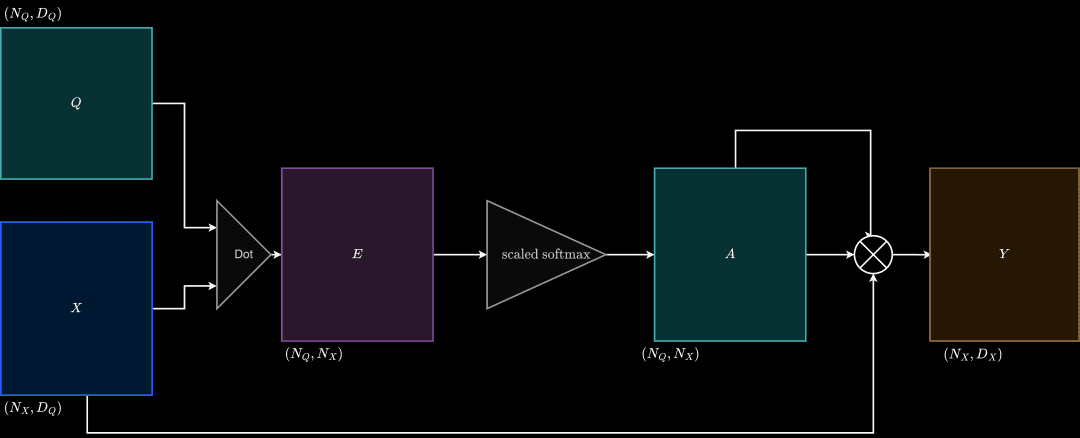
\includegraphics[width=\textwidth]{images/evolution-Version-3.png}
    \caption{Multihead Attention Versione 3}
\end{figure}

Nella $Versione \ 4$ si fanno dei cambiamenti nella versione di input. Si
divide l'input in coppie di matrici, rispettivamente \textbf{keys} e
\textbf{values}.
\begin{figure}[H]
    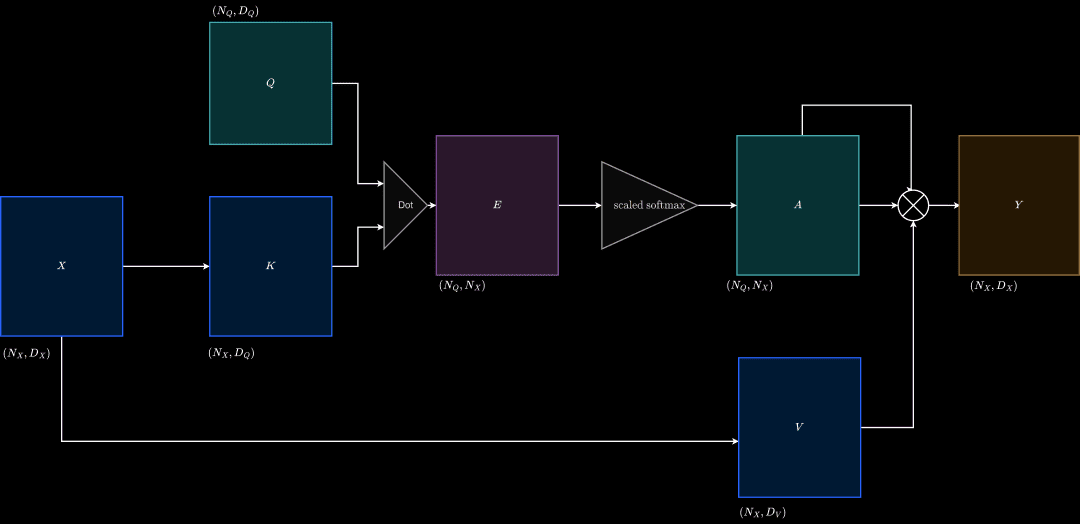
\includegraphics[width=\textwidth]{images/evolution-Version-4.png}
    \caption{Multihead Attention Versione 4}
\end{figure}

Per creare attenzione incrociata, apportiamo alcune modifiche. Le modifiche
sono specifiche della matrice di input. Come già sappiamo, l'attenzione
necessita di una matrice di input e di una matrice di query. Supponiamo di
proiettare la matrice di input in una coppia di matrici, vale a dire la matrice
chiave e quella valore .

La matrice chiave è curata rispetto alla matrice di query. Ciò si traduce in
pesi di attenzione. Qui la matrice dei valori viene trasformata con i pesi
dell'attenzione in contrapposizione alla trasformazione della matrice di input,
come visto in precedenza.

\begin{equation}
    \begin{aligned}
        K = X \cdot W_K \\
        V = X \cdot W_V \\
    \end{aligned}
\end{equation}

Questo viene fatto per disaccoppiare la complessità. La matrice di input può
ora avere una proiezione migliore che si occupa di costruire pesi di attenzione
e anche matrici di output migliori. La visualizzazione dell'attenzione
incrociata è mostrata nella Figura.

Nella $Versione \ 5$ fa riferimento alla $4$. Come abbiamo visto, ci sono 3
matrici: \textbf{Query, Keys, Values}. Sappiamo che le matrici keys e values
sono proiezioni delle matrici in input. E se facesimo come proiezione
dell'input anche la matrice di query?

\begin{equation}
    \begin{aligned}
        K = X \cdot W_K \\
        V = X \cdot W_V \\
        Q = X \cdot W_Q \\
    \end{aligned}
\end{equation}

\begin{figure}[H]
    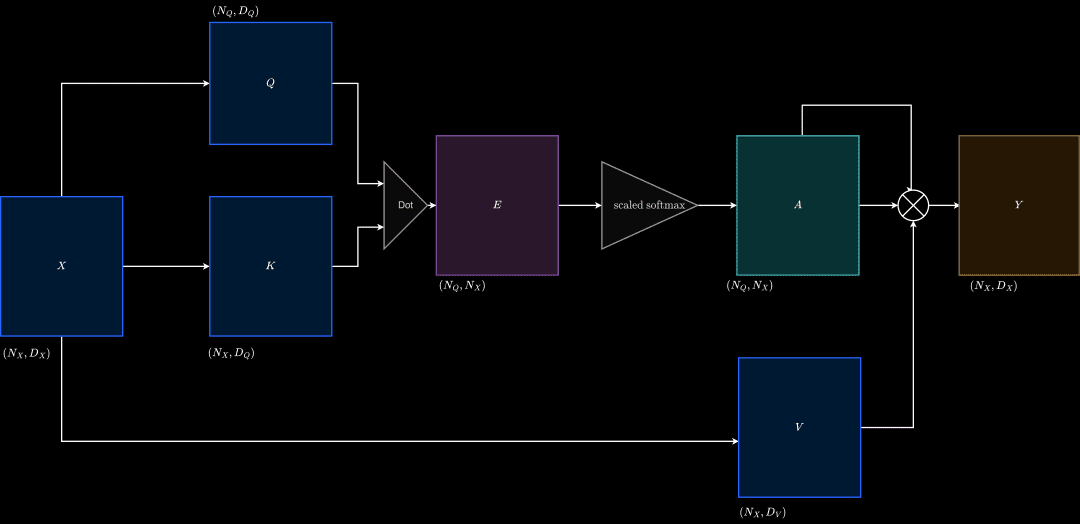
\includegraphics[width=\textwidth]{images/evolution-Version-5.png}
    \caption{Multihead Attention Versione 5}
\end{figure}

Nell'ultima versione, cioè la $Versione \ 6$, si parla di \textbf{multi-head
    attention}.

Le matrici di prima vengono proiettate ad un numero di teste. Gli splits
vengono passati ad un modulo di self attention, come abbiamo visto prima. Ogni
split viene poi \textbf{concatenato} in una singola rappresentazione.

\begin{figure}[H]
    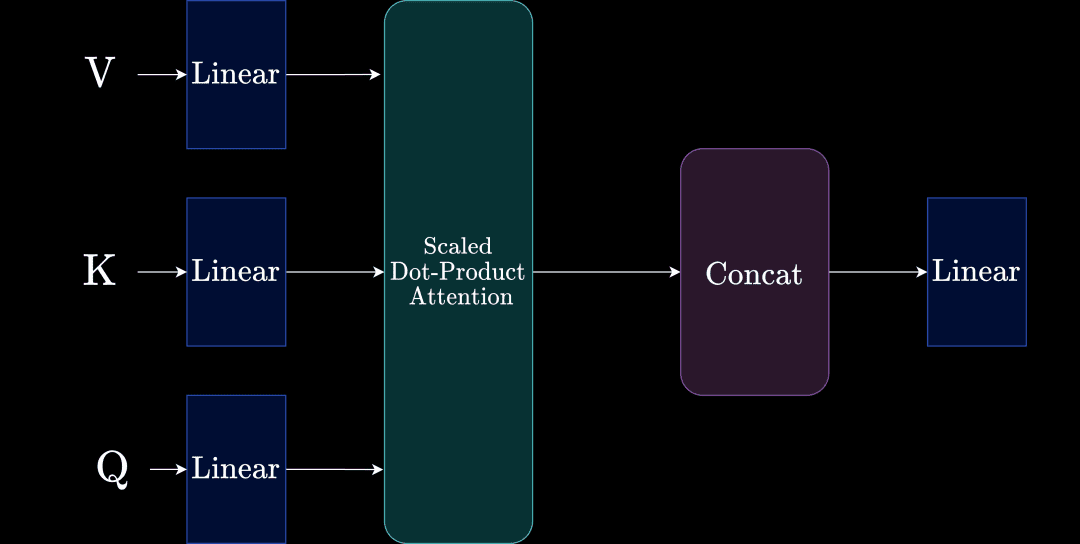
\includegraphics[width=\textwidth]{images/mha.png}
    \caption{Multihead Attention Versione 6}
\end{figure}

\subsection{Positional Encoding}

Se ci pensiamo, lavorando con matrici \textbf{non abbiamo il concetto di
    posizione} e di ordinamento. Per questo motivo, nell'architettura transformer
bisogna aggiungere l'informazione della posizione delle parole.

\begin{figure}[H]
    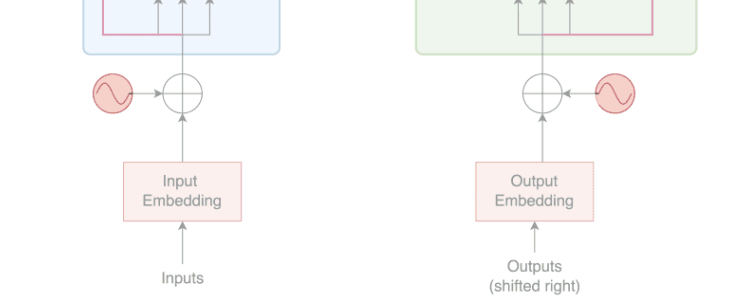
\includegraphics[width=\textwidth]{images/penc.png}
    \caption{Positional Encoding}
\end{figure}

Questi due nodi si occupano di aggiungere la posizione alla matrice di input.
In che modo, però? Per introdurlo, si sono usate 2 formule matematiche:

\begin{equation}
    \begin{aligned}
        PE_{pos, 2i} = sin \left( \frac{pos}{10000^{\frac{2i}{d_{model}}}} \right)   \\
        PE_{pos, 2i+1} = cos \left( \frac{pos}{10000^{\frac{2i}{d_{model}}}} \right) \\
    \end{aligned}
\end{equation}

Queste due sono le funzioni che vengono usate per aggiungere la posizione alla
matrice di input. \textbf{Ogni posizione} viene encodato in un
\textbf{vettore}.

\subsection{Come si allenano i transformers?}
Il concetto che si utilizza ormai è questo:

Transformer come BERT. Ecco una spiegazione più dettagliata di ciascuno dei
passaggi:

\begin{itemize}
    \item Si prende un dataset: Questo è il primo passo per l'allenamento di qualsiasi
          modello di machine learning. Il dataset dovrebbe consistere in una serie di
          esempi di testo. Per un modello di linguaggio, questo potrebbe essere un grande
          corpus di testo, come Wikipedia o un insieme di libri.
    \item Si creano delle coppie di testi (input con parole mascherate/nascoste, input):
          Questo passaggio descrive la creazione di esempi di allenamento per il modello.
          Per un modello come BERT, gli esempi di allenamento sono creati prendendo pezzi
          di testo dal dataset e mascherando alcune delle parole. Queste parole
          mascherate sono poi quelle che il modello cercherà di predire durante
          l'allenamento. Le coppie di testi quindi consistono nel testo con le parole
          mascherate (che funge da input per il modello) e il testo originale (che funge
          da "etichetta" o "obiettivo" per l'allenamento).
    \item Si fa l'allenamento per predire le parole mascherate/nascoste: Infine, il
          modello viene allenato per predire le parole mascherate basandosi sul contesto
          fornito dalle altre parole nell'input. L'obiettivo è che, dopo un sufficiente
          allenamento, il modello sarà in grado di utilizzare il contesto per "riempire
          gli spazi vuoti" in un pezzo di testo, il che è una competenza chiave per molte
          attività di elaborazione del linguaggio naturale.
\end{itemize}


Questi modelli \textbf{non sono fine-tunabili}. L'idea tipica non è fine tuning, ma \textbf{in context learning}.

\subsection{In Context Learning}

Immaginiamo di creare un app che ha un chatbot per un hotel. Le persone devono poterci interagire, richiedere camere, ecc\dots

\textbf{Scratch:} Fornire al sistema tutte le cose dellhotel. Costruire un transformer in base a questo.

\textbf{Usa un modello (Bert, GPT)}: Fornire il documento sul quale vuoi fare il fine tuning come prima frase di input del modello. Ad esempio, il documento di tutte le informazioni dell'hotel.

Ad esempio, scrivere per bene i passaggi nella richiesta del prompt fornisce risultati migliori e più precisi. 

Praticamente, non si programma niente e si inserisce solamente il contesto per salvarlo come stato del modello mentre lo si utilizza.
Si parla di \textbf{prompting engineering}.

\subsection{Few Shots learning}

Praticamente, in context learning ma oltre alla descrizione si forniscono degli \textbf{esempi} di quello che si vuole fare.
Questo per fare in modo per vedere se il modello riesce a generalizzare il problema e a risolvere il problema.
\newpage